%% v3.0 [2015/11/14]
%\documentclass[Proof,technicalreport]{ieicej}
\documentclass[technicalreport]{ieicej}
\usepackage[dvipdfmx]{graphicx}
\usepackage{here}
\usepackage[T1]{fontenc}
\usepackage{lmodern}
\usepackage{textcomp}
\usepackage{latexsym}
%\usepackage[fleqn]{amsmath}
%\usepackage{amssymb}
%\usepackage[dvipdfmx]{hyperref}
\usepackage{arabtex}
\usepackage{url}
\def\IEICEJcls{\texttt{ieicej.cls}}
\def\IEICEJver{3.0}
\newcommand{\AmSLaTeX}{%
 $\mathcal A$\lower.4ex\hbox{$\!\mathcal M\!$}$\mathcal S$-\LaTeX}
%\newcommand{\PS}{{\scshape Post\-Script}}
\def\BibTeX{{\rmfamily B\kern-.05em{\scshape i\kern-.025em b}\kern-.08em
 T\kern-.1667em\lower.7ex\hbox{E}\kern-.125em X}}
\jtitle{初級学習者を対象としたアラビア語検索サイトの構築}
\etitle{Developing Arabic Search Site to Help Beginner-level Learners}
\authorlist{%
 \authorentry[inoue.kai.n0@tufs.ac.jp]{井上 開}{Kai INOUE}{Tokyo}% 
 \authorentry[sano@tufs.ac.jp]{佐野 洋}{Hiroshi SANO}{Tokyo}% 
}
\affiliate[Tokyo]{東京外国語大学言語文化学部言語文化学科\hskip1zw
  〒183-8534 東京都府中市朝日町3-11-1}
 {Faculty of Engineering,
  Tokyo University of Foreign Studies\hskip1em
  3--11--1, Asahi-cho, Fuchu-shi, Tokyo,
  183--8534 Japan}
\affiliate[Tokyo]{東京外国語大学大学院総合国際学研究院\hskip1zw
  〒183-8534  東京都府中市朝日町3-11-1}
 {Tokyo University of Foreign Studies\hskip1em
  3--11--1, Asahi-cho, Fuchu-shi, Tokyo,
  183--8534 Japan}
%\MailAddress{$\dagger$hanako@denshi.ac.jp,
% $\dagger\dagger$\{taro,jiro\}@jouhou.co.jp}
\begin{document}
\setarab
%\novocalize
\begin{jabstract}
本研究は,初級学習者を対象としたアラビア語検索サイト構築について述べる.
近年日本でのアラビア語学習需要は高まりつつあるが,初級者の利用に主眼をおいた学習教材はまだ数が少ない.
アラビア語の辞書は,語根引きと基本形引きという2つの方法によって検索が可能である.
紙媒体ではどちらか一方しか採用できず,目的に応じて2冊の辞書を使い分ける必要性が生じる.
電子媒体の辞書によってこの問題を解決し、さらにスマートフォンからの利用への最適化や,初級レベルの語彙の選定という,既存の電子媒体辞書が抱える問題点の改善にも焦点を当てた.

\end{jabstract}
\begin{jkeyword}
アラビア語,辞書,検索サイト
\end{jkeyword}
\begin{eabstract}
This study reports developing search site for beginner-level learners.
Recently demand for leaning Arabic is getting higher in Japan, but the number of Arabic learning materials for beginner-level learners is still small.
The Arabic dictionary can be searched by two methods: root or basic form.
Because a paper dictionary cannoot adopt both of these two search ways at the same time, there is a necessity to use two dictionaries according to purpose.
We solved this problem with a dictionary of electronic media and also focused on improving the problems of existing electronic media dictionary such as optimization for use from smartphones and selection of vocabulary of biginner-level.

\end{eabstract}
\begin{ekeyword}
Arabic, search site, e-learning
\end{ekeyword}
\maketitle
\section{はじめに}
近年,日本ではアラビア語の学習需要が高まりつつある.
2011年,防衛省はアラビア語圏への留学派遣を開始し\cite{nikkei},2012年には東京外国語大学がアラビア語専攻の学部生募集定員を15名から30名へと増員した.
これらの背景には,日本おける21世紀以降のアラブ地域に対する政治的・経済的関心の高まりがある.
政治的には,2001年の「9.11」を始め,2003年からの「イラク戦争」,2010年からは「アラブの春」,翌年には「シリア内戦」の勃発,また「イスラム国」によるテロの脅威は現在も続いており,2014年にはシリアのアレッポで日本人2名が拘束された.
経済的には,原油輸入先第1位がサウジアラビア,第2位がアラブ首長国連邦,両国からの輸入量を合わせると全体の約6割を占めている\cite{teikoku}.
また日本企業の湾岸地域への進出も盛んである.
日本貿易振興機構が調査を始めた2005年から2014年の間に,アラブ首長国連邦にある日系企業拠点数は2倍以上の431事業所にまで増加している\cite{jetro}.
2020年にはドバイでの万国博覧会の開催が決定しており,湾岸地域はこれからますます経済的盛り上がりをみせると予想される.

しかし,日本でのアラビア語学習環境は,関心度の高まりに対してその充実度がまだ追い付いていない..
鷲見\cite{washimi2016}らによれば,2014年度にアラビア語の授業が開講されている大学は48あり,そのうち専門に学習できる教育課程が存在するのは大阪大学と東京外国語大学のみであり,残りの46の大学では副専攻の外国語として授業が開講されている.
現在日本の高等教育機関でアラビア語を学習する人口のほとんどが初級レベルにあるため,初学者用の学習教材の作成が必要である.
特に初学者用の辞書は数が少ない.
また紙媒体の初級者用辞書は基本形からの検索を採用していることが多く,語根を用いて語を調べることによる学習効果が期待できない.一方,これらの問題を解決した電子媒体の辞書は存在するものの,初学者向けに語彙が選定されていない点や,スマートフォンでの利用に特化されていない点などが問題である.

本研究では,『『大学のアラビア語』』単語帳』および『A Frequency Dictionary of Arabic』のデータを用いて,アラビア語辞書検索サイトを構築した.基本形からの検索と語彙検索とを両立させつつ,これらのデータを用いて語彙を初級者向けに選定した.またスマートフォンからの利用に最適化したプラットフォームにすることで利便性も追求している.

\section{アラビア語の言語的特徴}
アラビア語は,アフロ・アジア語族のセム語派に属する言語である.アラビア語はエジプトやシリアをはじめ,20以上の国および地域で公用語となっている.
Ethnologue\footnote{\url{https://www.ethnologue.com/statistics/size}}によると,話者総人口はおよそ3億人にものぼると言われ,また6つある国連公用語の1つにも数えられる.
アラビア語はイスラム教の聖典であるコーランの言語であり,全世界およそ16億人のイスラム教徒が存在することを考慮に入れると,実に世界人口の5人に1人がアラビア語と関わりを持っていることとなる.

文字はアラビア文字を用い,右から左に向かって記述する一方,数字は逆に右から左に記述される.
28の子音が存在し,中でも咽頭化ないし軟口蓋音化した子音が特徴的である.
母音は/a/,/i/,/u/の短母音とそれぞれの長母音,また/ai/,/au/などの二重母音が弁別される.
文構造はVSO型が基本だが,SVO型を取ることも多い.
名詞と形容詞は格(主格,属格,体格)・性(男性,女性)・数(単数,双数,複数)によって変化し,定冠詞によって限定と非限定が区別される.
また複数形には規則形が存在するが,不規則変化するものが多数である.
名詞と形容詞では,単数形が基本形である.
動詞は人称(一人称,二人称,三人称)・性・数,および完了と未完了によって変化する.
動詞では,三人称男性単数完了形が基本形である.

アラビア語は,3子音を語根とすることが形態論的特徴である.
語根とは基本的な意味を持つ最小単位のことであり,語から派生接辞と屈折接辞を取り除いた部分を指す\cite{nishihara2012}.
アラビア語の場合,一般的な意味での語根からさらに母音が取り除かれた部分のことを指す.
またHabash\cite{habash2010}は,「語根は,その全ての派生語によって共有されるいくつかの抽象的な意味を示す」と説明している.
アラビア語において語根が単体で語となることはないが,それぞれの語根には固有の意味が備わっており,同じ語根から派生した語は意味に関連性をもっている.

\begin{table}[ht]
\begin{center}
\begin{tabular}{l|ccc}
   語根& <b>-<t>-<k> & \textit{\textbf{k}-\textbf{t}-\textbf{b}} & 《書くこと》\\
  \hline
 派生語& <kAtibuN> & \textit{\underline{\textbf{k}}A\underline{\textbf{t}}i\underline{\textbf{b}}\~u} & 作家\\
  派生語& <kitAbuN> & \textit{\underline{\textbf{k}}i\underline{\textbf{t}}A\underline{\textbf{b}}\~u} & 本\\
\hline
\end{tabular}
\caption{語根<b>-<t>-<k> \textit{\textbf{k}-\textbf{t}-\textbf{b}}《書くこと》とその派生語.派生語内の語根は,下線で示されている.}
\label{table:alignment}
\end{center}
\end{table}

例えば,<kAtibuN> \textit{\underline{\textbf{k}}A\underline{\textbf{t}}i\underline{\textbf{b}}\~u}\footnote{本稿では,アラビア文字をHabash-Soudi-Buckwalter記法\cite{hsb}に従って転記する.} は「作家」を意味し, <kitAbuN> \textit{\underline{\textbf{k}}i\underline{\textbf{t}}A\underline{\textbf{b}}\~u}は「本」を意味する.
両単語の語根は<b>-<t>-<k> \textit{\textbf{k}-\textbf{t}-\textbf{b}}であり,これは《書くこと》にまつわる語根である.
ここで注意したいのは,語根はその並べ方まで含めたものであり,語根<b>-<t>-<k> \textit{\textbf{k}-\textbf{t}-\textbf{b}}は,<k>-<t>-<b> \textit{\textbf{b}-\textbf{t}-\textbf{k}}や<t>-<b>-<k> \textit{\textbf{k}-\textbf{b}-\textbf{t}} とは異なる.\footnote{3つの子音の順列が全て語根となるわけではない.}
厳密に言えば,3子音の組み合わせではなく,3子音の順列であると言える.
また稀に4子音の語根も存在する.

\section{アラビア語辞書検索システムの構築}
\subsection{既存辞書の問題点}
紙媒体の初学者用の辞書としては,「パスポート初級アラビア語辞典」がある.
これは約4,200語を収録した基本形から検索する辞書である.
意味の選定や補足が充実した辞書であるが,辞書の利用のしやすさをとって基本形からの検索を採用したことで,後述する語根からの検索によって期待される学習効果が得られない.

一方,語根からの検索と基本形からの検索との両立が可能な電子媒体の辞書としては「アラビア語検索エンジン アラジン\footnote{http://www.linca.info/alladin/}」が有名である.
莫大な語彙データを収録しており,動詞活用形や名詞複数形からも語を検索することができる.
しかし,それらを列挙する形で検索結果が表示されるため,必ずしも利用者が探している語彙とのマッチがとられるわけではない.
莫大な語彙を収録しているがために,初学者にとっては語彙データが選定されていないという問題がある.

またパソコンからの利用を想定しているため,スマートフォンの小さい画面では利用しづらいという問題もある.
LINEの調査\footnote{https://linecorp.com/ja/pr/news/ja/2017/1819}によれば,日常的にインターネットを利用する際,85\%の人がスマートフォンを利用しており,そのうちスマートフォンのみを利用している人の割合は全体の約半数にも及ぶ.
特に若年層ではその傾向が如実である.
大学でアラビア語を学習する人の大半は,10代と20代であると考えられるため,アラビア語検索サイトを使う際はスマートフォンから利用すると推測される.
学習者のインターネット利用環境に最適化させることも,課題の1つとなる.

\subsection{語根・基本形からの検索}
\subsubsection{語根からの検索}
伝統的にアラビア語の辞書では,語根から語を検索する辞書が主流であった.
表1の例であれば,<kAtibuN> \textit{\underline{\textbf{k}}A\underline{\textbf{t}}i\underline{\textbf{b}}\~u}と<kitAbuN> \textit{\underline{\textbf{k}}i\underline{\textbf{t}}A\underline{\textbf{b}}\~u}はともに辞書の見出し語<b>-<t>-<k> \textit{\textbf{k}-\textbf{t}-\textbf{b}}のグループにまとめられている.
今まで基本形から語を検索する日本語や英語の辞書しか使ったことのない学生が,語根から検索するアラビア語辞書の利用に慣れるまでには時間を要する.
また語根から語を検索するためには,調べたい語の語根を判別する必要性があり,これには相応の文法能力が必要とされる.

\begin{table}[ht]
\begin{center}
\begin{tabular}{l|ccc}
   語根 & <b>-<t>-<k> &\textit{\textbf{k}-\textbf{t}-\textbf{b}}& 《書くこと》\\
  \hline
 派生語 & <maktabaTuN>&\textit{ma\underline{\textbf{k}}\underline{\textbf{t}}a\underline{\textbf{b}}a$\hbar$\~u} & 図書館\\
\hline
\end{tabular}
\caption{語根<b>-<t>-<k> \textit{\textbf{k}-\textbf{t}-\textbf{b}}《書くこと》とその派生語<maktabaTuN> \textit{ma\underline{\textbf{k}}\underline{\textbf{t}}a\underline{\textbf{b}}a$\hbar$\~u}「図書館」}
\label{table:alignment}
\end{center}
\end{table}

例えば,「\textit{ma\underline{\textbf{k}}\underline{\textbf{t}}a\underline{\textbf{b}}a$\hbar$\~u}」を辞書で引く場合,「\textit{m}」と「\textit{t}」がそれぞれ語根ではなく,派生語を作るための接辞であると見抜けなければならない.
これは簡単な例であるが,語根の中には派生された語において3子音のうち一部が脱落したり,変化したりするものがある.
これらは例外だが,使用頻度の高い重要語にも数多く見られる.

\begin{table}[ht]
\begin{center}
\begin{tabular}{l|ccc}
   語根 & <m>-<w>-<n>&\textit{\textbf{n}-\textbf{w}-\textbf{m}} & 《寝ること》\\
  \hline
 派生語& <nAma>&\textit{\underline{\textbf{n}}A\underline{\textbf{m}}a} & 寝る\footnotemark\\
  派生語& <niyAmuN>&\textit{\underline{\textbf{n}}iyA\underline{\textbf{m}}\~u} & 睡眠\\
\hline
\end{tabular}
\caption{語根 <m>-<w>-<n> \textit{\textbf{n}-\textbf{w}-\textbf{m}}《寝ること》とその派生語.}

\label{table:alignment}
\end{center}
\end{table}
\footnotetext{三人称男性単数完了形.}
「NWM」は「寝る」に関わる語根だが,これが派生した動詞「{\underline{\textbf{n}}A\underline{\textbf{m}}a}」では第二子音「W」が長母音化し,名詞「\textit{\underline{\textbf{n}}iyA\underline{\textbf{m}}\~u}」では同じく第二子音「W」が「Y」に変化している.
これらの例のように,一見しただけでは語根の判別が難しい語も多い.
こういった場合,語根から辞書を引くことは格段に難しくなる.
特に文法能力がまだ十分に備わっていない初学者は,語の意味を調べることさえできないという状態に陥る.
これが語根を用いて検索する辞書の大きなデメリットである.
しかし,逆に語根を正しく判別するだけの文法能力さえあれば,同じ語根から派生された語彙を一覧することができるというメリットもある.
<b>-<t>-<k> \textit{\textbf{k}-\textbf{t}-\textbf{b}}を引けば,「作家」,「本」,「図書館」という語を同時に知ることができる.
また動詞の活用形や名詞・形容詞の複数形を基本形に戻すことができないとしても,語根から辞書を引くことで意味を知ることが可能である.

\begin{table}[ht]
\begin{center}
\begin{tabular}{l|ccc}
   語彙 & 意味 & 複数形\\
  \hline
  <kAtibuN> \textit{\underline{\textbf{k}}A\underline{\textbf{t}}i\underline{\textbf{b}}\~u} & 作家 & <kuttAbuN> \textit{\underline{\textbf{k}}\underline{\textbf{t}}A\underline{\textbf{b}}\~u} \\
  <kitAbuN> \textit{\underline{\textbf{k}}i\underline{\textbf{t}}A\underline{\textbf{b}}\~u} & 本 & <kutubuN>  \textit{\underline{\textbf{k}}u\underline{\textbf{t}}u\underline{\textbf{b}}\~u} \\
\hline
\end{tabular}
\caption{語根KTBと派生語「本」「作家」の複数形}
\label{table:alignment}
\end{center}
\end{table}

語根から引く辞書であれば,「\textit{\underline{\textbf{k}}A\underline{\textbf{t}}i\underline{\textbf{b}}\~u}」が「\textit{\underline{\textbf{k}}A\underline{\textbf{t}}i\underline{\textbf{b}}\~u}」の複数形であると知らなくとも,語根が「<b>-<t>-<k> \textit{\textbf{k}-\textbf{t}-\textbf{b}}であるということさえわかれば,辞書を引いて意味を知ることできる.
「\textit{\underline{\textbf{k}}u\underline{\textbf{t}}u\underline{\textbf{b}}\~u} 」に関しても同様であり,これらの語はいずれも語根に対して母音が付加されているだけなので,語根の判別は難しくない.
それゆえ語根から引く辞書であれば,たとえこれらの語が初見であったとしても辞書を引くことは可能である.

\subsubsection{基本形からの検索}
語根から検索する辞書がある一方で,日本語や英語の辞書と同様に基本形から検索する辞書も存在する.
この場合,調べたい語の語根を判別できる文法能力は必要とならないため,初学者にとっては使い勝手がよいというメリットがある.
<m>-<w>-<n> \textit{\textbf{n}-\textbf{w}-\textbf{m}}のように派生語において語根の一部が,欠落および変化してしまう語も,単純にそのままの形で調べれば良い.
しかし一点注意しなければいけない点がある.
名詞・形容詞は単数形,動詞は三人称男性単数完了形が基本形となっているため,調べたい語彙が名詞・形容詞の複数形だった場合や,動詞の活用形だった場合や,それらを基本形に戻す文法能力が必要である.

表4の例であれば,「\textit{\underline{\textbf{k}}\underline{\textbf{t}}A\underline{\textbf{b}}\~u}」は「\textit{\underline{\textbf{k}}A\underline{\textbf{t}}i\underline{\textbf{b}}\~u} 」に,「\textit{\underline{\textbf{k}}u\underline{\textbf{t}}u\underline{\textbf{b}}\~u} 」は「\textit{\underline{\textbf{k}}i\underline{\textbf{t}}A\underline{\textbf{b}}\~u}」に戻さなければ辞書を引くことはできない.
複数形が規則変化するものである場合,複数形から単数形を復元することは難しくないため,基本形から引く辞書ですぐに調べることができる.
しかし表4の名詞のように複数形が不規則変化するものの場合,辞書を引くのは当然それらが学習者にとって初見の時であるため,複数形から単数形への復元は困難であり,辞書を引くことは難しくなる.
この場合には,語根から検索する方が適当である.
また同じ語根から派生された語彙を一覧することができないため、辞書を引くという行為が新たな語を学ぶという部分に結びつかない。初学者にとって語根から検索することは難しいが,同時に多くの語を覚えなければいけない学習初期にこそ語根から語を調べることが効率的である.

\subsubsection{検索方法の検討}
語根検索と基本形検索にはそれぞれに長所と短所がある.

語根検索には,同じ語根から派生した語彙を一覧できることや,語を基本形に戻せなくても検索できるといったメリットが存在する.
特に前者に関しては,語を調べつつ新たな語を学ぶことができ,高い学習効果が期待できる.
一方で語の語根を見抜く文法能力が要求されることが最大のデメリットであり,これは初学者にとって大きな障害となる.

基本形検索では,語根に関する知識がなくても辞書を利用できるため,初学者にも利用しやすいことが最大のメリットとなる.
しかし,今度は調べたい語を基本形に戻せるだけの文法能力が要求される.

初学者にとっての使いやすさのみを考慮すれば,基本形検索を採用することが妥当であるが,語根検索によって得られる学習効果も大きい.アラビア語辞書において伝統的に語根検索が採用されてきたことは,語根に対する理解がアラビア語学習において重要であるからに他ならない.しかし榮谷\cite{sakaedani2008}も指摘するように,語根を重視して文法学習に重点をおけば,かえって語彙を覚える時間が取れなくなるという可能性もある.

紙媒体の辞書では,物理的にどちらか一方の検索方法しか採用できないため,目的に応じて使い分けようとすれば2冊必要となってしまう.
他方電子媒体の辞書であれば両方を採用することができる.
電子媒体のアラビア語辞書をつくることのメリットの1つは,この点にある.
本論で構築する辞書検索サイトも語根検索と基本形検索を備えている.

\subsection{アラビア語辞書データ}
我々は,収録する語彙データとして『『大学のアラビア語』』単語帳』\cite{aoyama2015}より2,081語を抽出した.
これは,大学でアラビア語を学ぶ人が覚えるべき語彙を収録したものである.
さらに『A Frequency Dictionary of Arabic』の上位2,000語のうち,『『大学のアラビア語』』単語帳』に含まれない818語を追加した,最終的に全2,909語を収録した.
またTufs言語モジュール\cite{kawaguchi2007}にアップロードされている約2,000文を例文として収録した.

3.1で取り上げたように,語彙数をむやみに増やせば初学者にとって検索結果の中から適切なものを選び出すのが困難となる.
そのため本稿で構築する辞書建築サイトでは,語彙数に制限を設けた.
では初学者にとって最低限必要となる語彙数はどの程度の量になるのか.
第二言語習得においてどれだけの語彙量を目標にすべきかに関して,Nation\cite{nation1990}は語彙の頻度に注目することを1つの方法として挙げている.
彼は英語ネイティブスピーカーの中等学校教科書を例に,最も頻度の高い2000語でテキストの87\%,さらにUniversity word list\footnote{英語において最も頻度の高い2000語を除き,学術文書において最も頻度の高い約800語のこと.\url{http://jbauman.com/aboutUWL.html}}を加えた2800語でテキストの95\%をカバーしていると示している.
この結果は英語に限られるものであり,他言語にも同じように頻度とテキストカバー率の関係を当てはめるべきではない.

しかしBuckwalterら\cite{buckwalter2009}が,語彙学習において頻度を1つの指標とした際,多くの場合学習者の利益となる語彙表を得られると述べているように,頻度が重要な指標となることは間違いない.
とりわけ「初学者が学ぶべき語彙を提示する」という条件のもとでは,効果的だと考えられる.

\subsection{実装詳細}
本研究で構築した検索サイトの仕様を表\ref{table:website}に示す.
検索サイトは,スマートフォンからの利用に最適化されているが,パソコンからでも使用できる.
また,推奨ブラウザにないInternet Explorerからも使用できるが,一部画面表示が変更される.

\begin{table}[ht]
\begin{center}
\begin{tabular}{l|p{6 cm}}
   媒体 & ウェブサイト\\
  \hline
    対応機種 & スマートフォン,パソコン\\
    推奨ブラウザ & Firefox,GoogleChrome,Safari\\
    言語 &  アラビア語,日本語\\
    仕様対象者 &  日本語を母語とするアラビア語の初級学習者\\
    検索方法 &  見出し語検索,語根検索,日本語検索\\
    記載文法事項 &  語,品詞,語根,意味,派生語,例文\\
    収録語彙 &  2,909語\\
    辞書データ &  『『大学のアラビア語』単語帳』,『A Frequency Dictionary of Arabic』,Tufs言語モジュールアラビア語(例文)\\
\hline
\end{tabular}
\caption{検索サイト仕様}
\label{table:website}
\end{center}
\end{table}

検索サイトには,基本形検索,語根検索,および日本語検索が備わっている.基本形検索,語根検索ではアラビア語,日本語検索では日本語をテキストボックスに入力する.
基本形検索と語根検索では,テキストボックスへの入力と語彙データのマッチングが完全一致で行われ,日本語検索では部分一致でマッチングが行われる.
検索ボタン/searchボタンないしEnterをクリックすると,検索結果が表示される.
消去/デリートボタンをクリックすることで,テキストボックス内の入力が消去される.

\begin{figure}[H]
\begin{center}
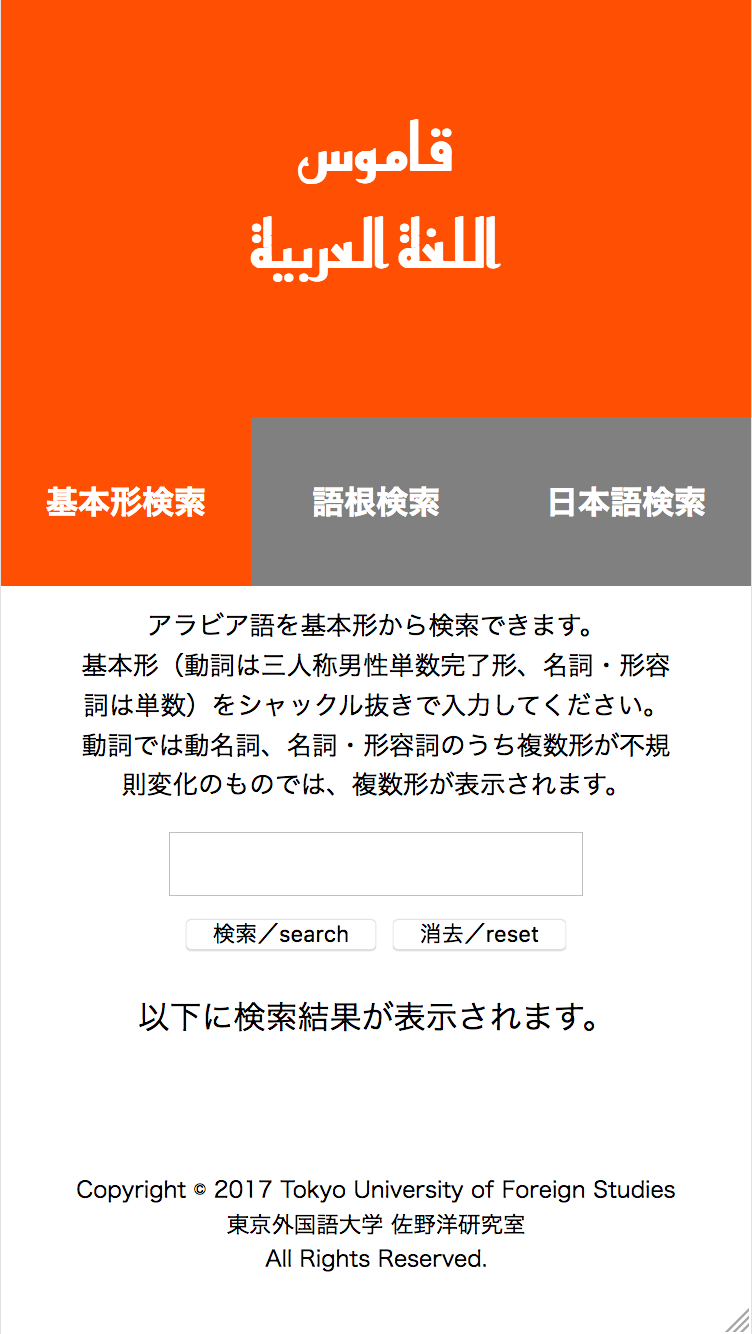
\includegraphics[scale=0.4]{fig01.png}
\caption{インデックス画面}
\end{center}
\end{figure}

また検索ボックスには,入力補完機能が実装されており,収録されている語彙データが検索候補として表示される仕様になっている.
検索したい語の基本形や語根が曖昧な場合にも,検索候補を表示することによって利用者の探している語とのマッチングが取れる可能性を高めている.

図2のように,基本形検索において<k> \textit{k}と入力すると,語彙データにある<k> \textit{k}から始める語が検索候補として表示される.

\begin{figure}[H]
\begin{center}
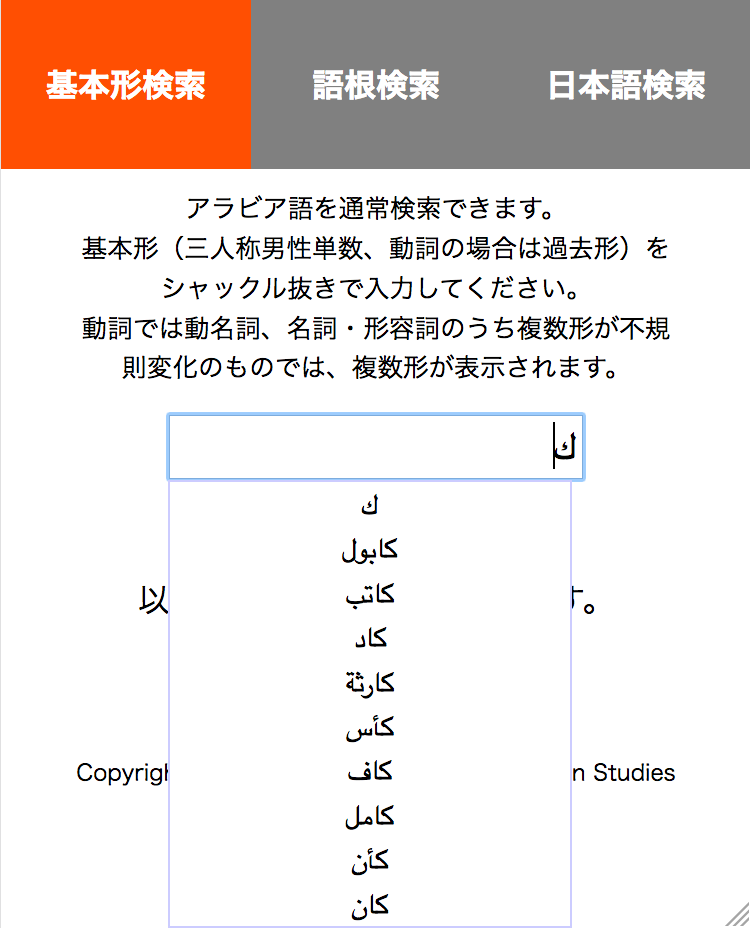
\includegraphics[scale=0.4]{fig02.png}
\caption{入力補完}
\end{center}
\end{figure}

辞書サイトの画面表示はスマートフォンから利用に最適されている.
語根検索で複数の語が検索結果として表示される場合などには,画面に下にスクロールしていくことで検索結果をみることができる.
個々の語に関する情報は画面左側にテーブル形式で表示される.
表示される情報は順に,語,品詞,語根,意味,派生語、例文である.
派生語は,動詞の動名詞,ないし名詞・形容詞の不規則変化する複数形である.
派生語と例文は,該当するデータがない場合には表示されない.
また例文はその他の語の情報の下段に表示される.

\begin{figure}[H]
 \begin{minipage}{0.5\hsize}
  \begin{center}
   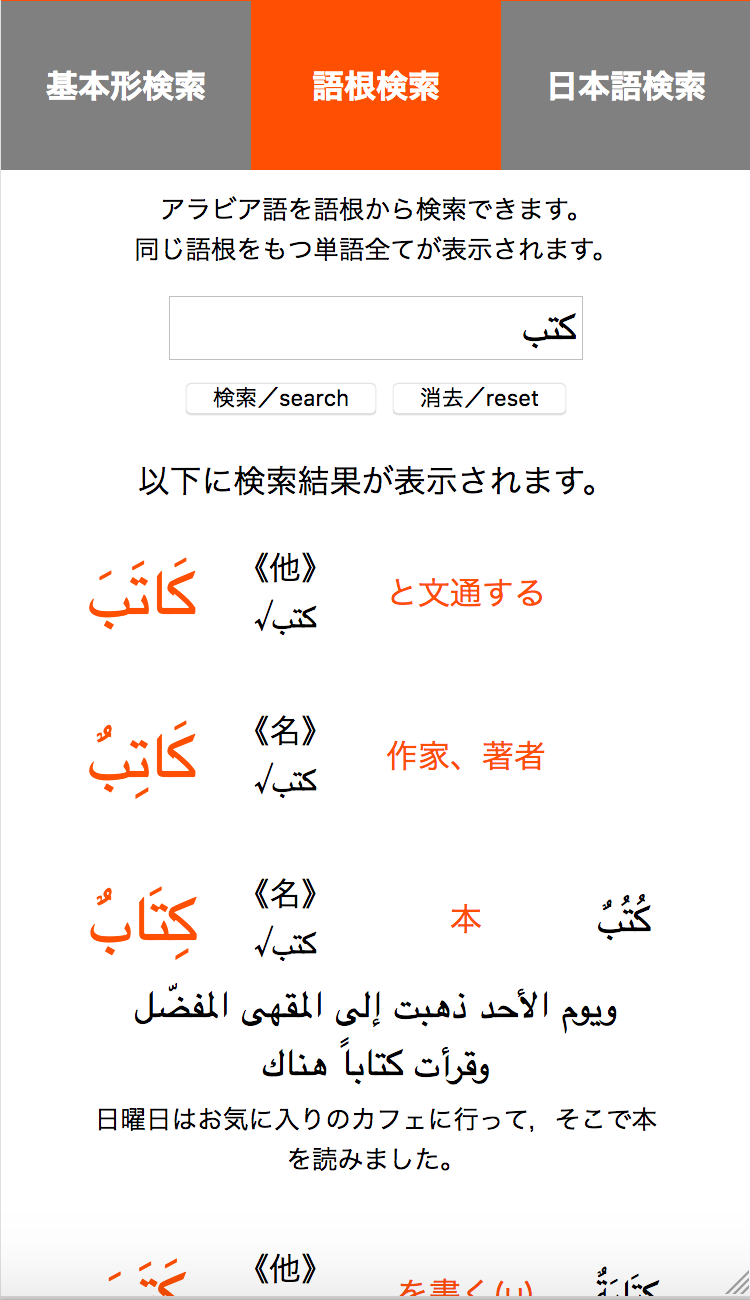
\includegraphics[scale=0.3]{fig03.png}
  \end{center}
  \caption{語根KTBの検索結果1}
 \end{minipage}
 \begin{minipage}{0.5\hsize}
  \begin{center}
   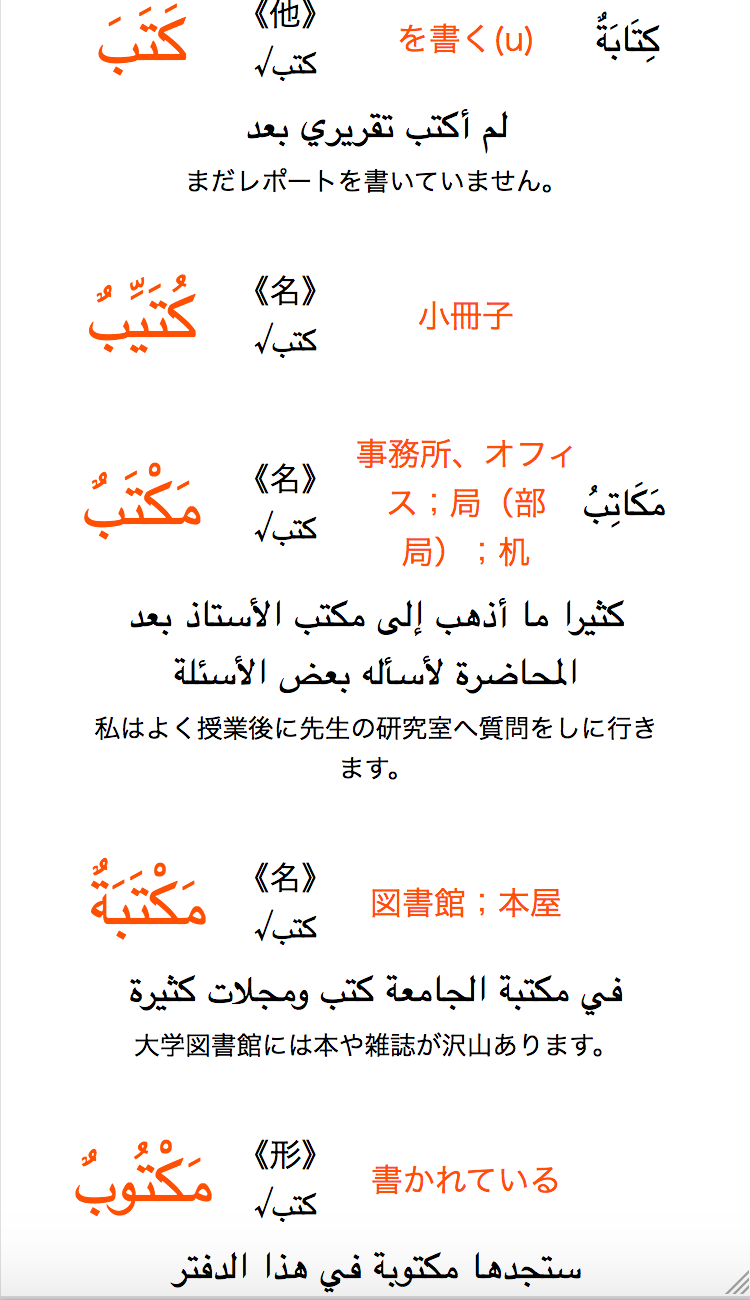
\includegraphics[scale=0.3]{fig04.png}
  \end{center}
  \caption{語根KTBの検索結果2}
 \end{minipage}
\end{figure}

\section{おわりに}
本研究では,『『大学のアラビア語』』単語帳』および『A Frequency Dictionary of Arabic』を用いて初級学習者向けのアラビア語辞書検索サイトを構築した.
これらの語彙データを用いることで,語彙を初級者向けに選定している.
検索サイトは,基本形からの検索と語彙からの検索の2つを兼ね備えており,またスマートフォンからの縦長の画面から利用の最適化されている.

検索サイトでは初学者向けに語彙を選定するため,頻度を1つの指標とし,上位2,000語までを収録した.
これが初学者の学習目的や能力に見合ったものである保証はなく,実際に検索サイトが利用されていく中で調整する必要がある.
また純粋に頻度のみを指標としたが、仕様頻度は高くないが日常的によく用いる語彙などが不足している可能性もある.
これらを踏まえ,収録する語彙とその量を調整していくことが今後の大きな課題となる.

\section{謝辞}
本研究で用いた語彙データの一部は,東京外国語大学の青山弘之氏から提供を受けた.
また論文執筆において奈良先端技術大学院大学の井上剛氏から多くの助言をいただいた.

\begin{thebibliography}{99}
\bibitem{washimi2016}
鷲見朗子 鷲見克典, 日本の高校と大学におけるアラビア語の教育と学習者, アラブ・イスラム研究(14), pp.103-121, 2016.
\bibitem{habash2010}
Nizar Habash,Introduction to Arabic Natural Language Processing,Morgan\&Claypool,2010.
\bibitem{hsb}
Nizar Habash, Abdelhadi Soudi, and Tim Buckwalter,On Arabic Transliteration,Arabic Computational Morphology: Knowledge-based and Empirical Methods,Springer,2007.
\bibitem{nishihara2012}
西原哲雄,言語学入門,朝倉書店,2012
\bibitem{sakaedani2008}
榮谷温子,アラビア語辞典の語根順配列とアルファベット順配列語彙習得の観点から, 外国語教育研究(11),pp.90-100,2008.
\bibitem{aoyama2015}
青山弘之,イハーブ・アフマド・エベード,『大学のアラビア語』単語帳,東京外国語大学,2015.
\bibitem{heinle1990}
I.S.P.Nation,Teaching and Learning Vocabulary, Heinle\&Heinle,1990.
\bibitem{buckwalter2009}
Tim Buckwalter,Parkinson Dilworth,A Frequency Dictionary of Arabic: Core Vocabulary for Learners, Routledge,2009.
\bibitem{kawaguchi2007}
Yuji Kawaguchi,Toshihiro Takagaki,Nobuo Tomimori,and Yoichiro Tsuruga,
Corpus-Based Perspectives in Linguistics,John Benjamins,2007.
\bibitem{teikoku}
「原油の生産トップ10と日本の輸入先」, \textless \url{https://www.teikokushoin.co.jp/statistics/map/index16.html}\textgreater,2017年2月26日アクセス.
\bibitem{jetro}
 日本貿易振興機構(ジェトロ),「日本の企業」\textless \url{https://www.jetro.go.jp/ext_images/_Reports/02/8a510d662cfc29f9/6_jpcompany.pdf}\textgreater,2018年2月26日アクセス.
\bibitem{nikkei}
「アラビア語の専門家を育成」\textless \url{https://www.nikkei.com/article/DGXNZO22129830T20C11A1PE8000/}\textgreater,2018年2月26日アクセス.
\end{thebibliography}
\end{document}